\begin{frame}{The NEMO ORCA12 Ocean Model~\cite{madec2015nemo}}
\vspace{-20pt}
\begin{figure}[htb!]
    \centering
    \hspace{-30pt}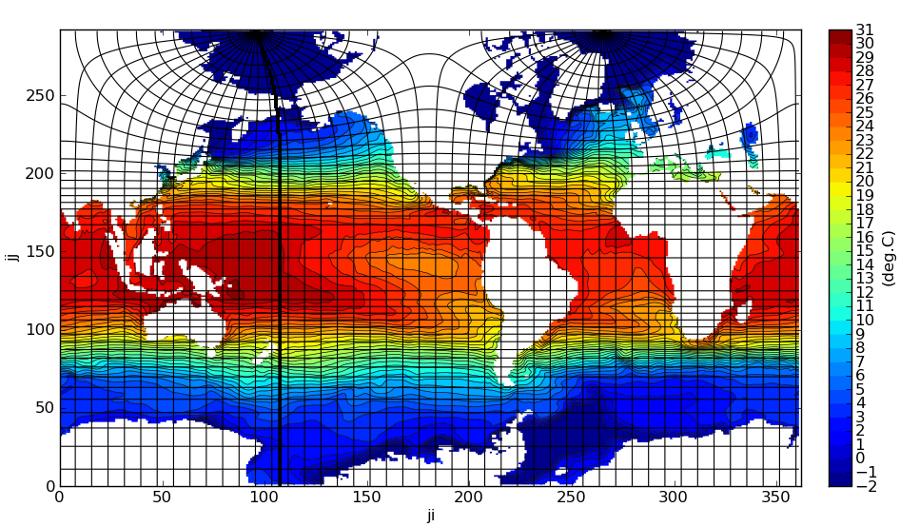
\includegraphics[width=0.74\linewidth]{images/example-images/fig-irregular.png}
     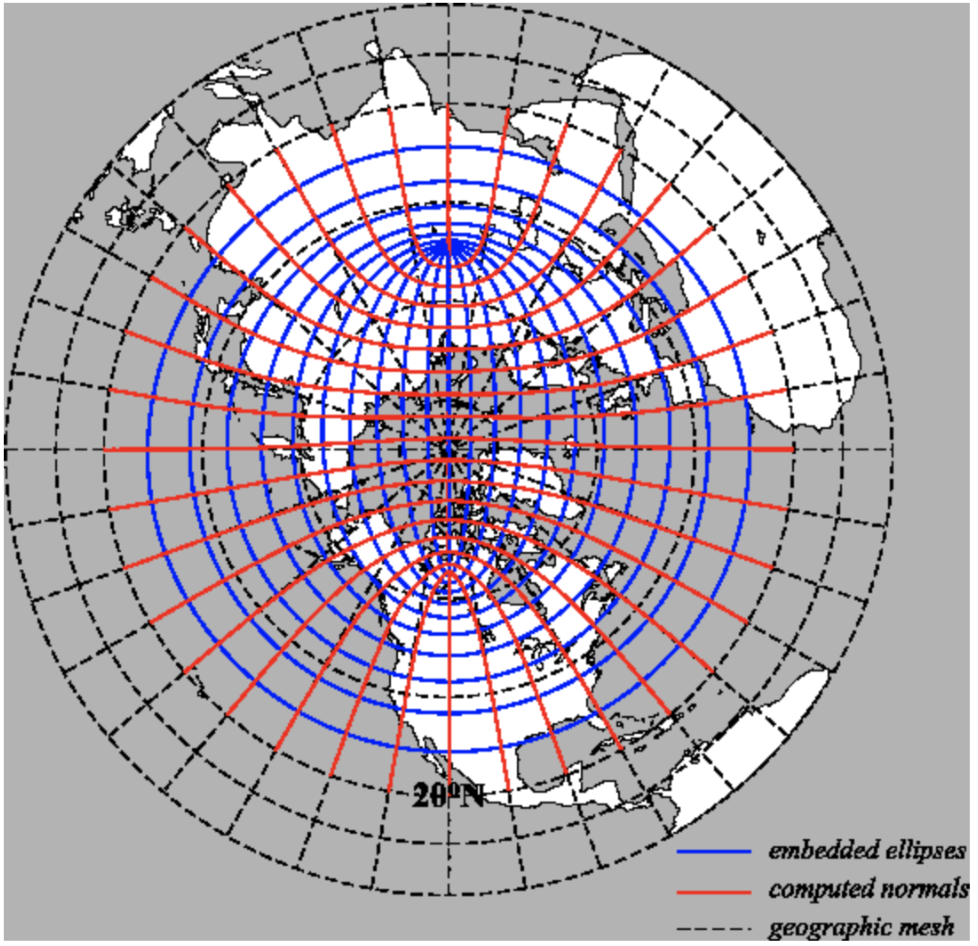
\includegraphics[width=0.30\linewidth]{images/example-images/nemo-poles.png}
    \vspace{-7pt}
    \caption{NEMO ORCA12 uses a tripolar ocean grid so that no coordinate singularities are in the ocean.
     The resolution is $\frac{1}{12}^{\circ}$.
      Initial condition EN4~\cite{good2013en4, HadObs} (start of the run = 1976).
Forcing CORE2~\cite{griffies2012datasets,large2009global}.}
    \label{fig:}
\end{figure}
\end{frame}


\begin{frame}{The HADGEM3 CMIP6 Model~\cite{williams2018met, FurtherInfo}}
\vspace{-25pt}
\begin{itemize}
\item `\texttt{control-1950}' to 2050. Daily mean outputs~\cite{williams2018met, FurtherInfo}.\footnote{\url{https://view.es-doc.org/
                                                ?renderMethod=name&project=cmip6&type=
                                                cim.2.designing.NumericalExperiment&client
                                                =esdoc-url-rewrite&name=control-1950}}

\item This experiment is not standard to CMIP6~\cite{eyring2016overview}.
\item There is a problem with representing TCs~\cite{tomassini2017interaction}:
\end{itemize}
\begin{figure}
\vspace{-18pt}
        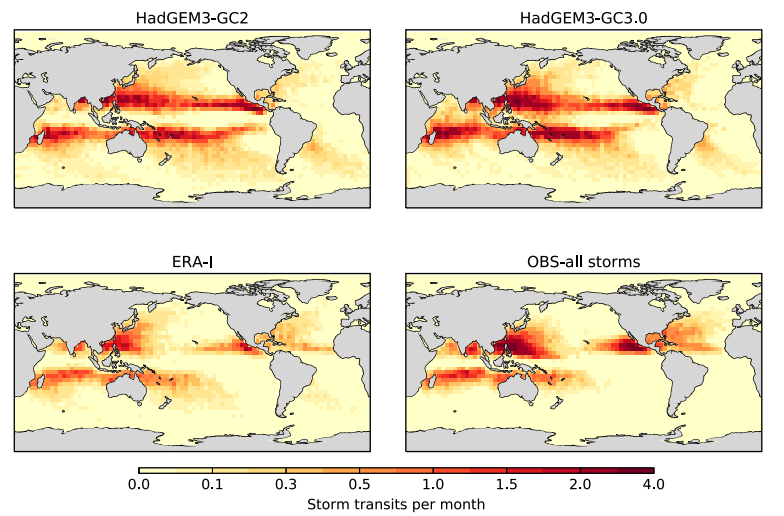
\includegraphics[width=0.7\linewidth]{images/HAD-TC.png}
\vspace{-10pt}
            \caption{The models all have
            significantly less TCs in the North Atlantic
             than observations.
             \textit{Figure 19 from~\cite{williams2018met}.} }
\end{figure}
\vspace{-15pt}
\end{frame}

\begin{frame}{Systematic Error: Wind Stress Parameterisation}
\vspace{-40pt}
\centering
\begin{equation}
 |\tau| = C_d(|U|) \cdot U^2
 \end{equation}
    \hspace{-30pt}\begin{minipage}{0.45\textwidth}
    \begin{figure}
            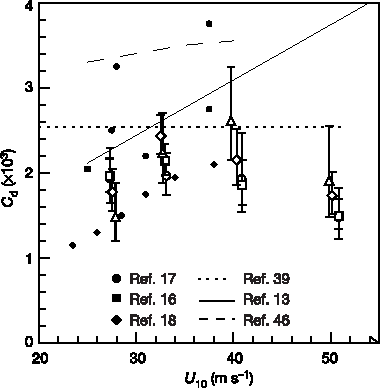
\includegraphics[width=1\linewidth]{images/example-images/cd.pdf}
                \caption{Fig. 3c from Powell 2003~\cite{powell2003reduced},
                 where they suggested that at high wind speeds $c_d$ decreases.}
    \end{figure}
    \end{minipage}\hspace{5pt}
      \begin{minipage}{0.57\textwidth}
\begin{figure}[htb!]
    \centering
    \includegraphics[width=1\linewidth]{../surge/plots/cd_finder.pdf}
    \caption{ Extracting $C_d$ from data.
    $ r_p = 0.9774 \pm 0.001,\;\; p<10^{-300}$\\
    $ m = 0.0383 \pm 0.0001 $ kg$^{0.5}$ m$^{-1.5}$\\
    $\implies  c_d = 0.001467 \pm 0.000008$ kg m$^{-3}$
    % error estimated from differences in output between test/training year,
    % measured regression error in either year much smaller than this.
    % The error is propogated using the \texttt{python3.uncertanties} package}
    There might be a theoretical limit~\cite{donelan2004limiting}.
    }
    %\label{fig:}
\end{figure}
    \end{minipage}
\end{frame}
